\documentclass[a4paper, 12pt]{article}

\usepackage[T1]{fontenc}
\usepackage[utf8]{inputenc}
\usepackage[english]{babel}  % ngerman for German
\usepackage{lmodern}  % nicer font
\usepackage{geometry}
\geometry{%
	left   = 2.5cm,
	right  = 2.5cm,
	top    = 3cm,
	bottom = 3cm
}

\usepackage{textcomp}
\usepackage{gensymb}
\usepackage{amsmath,amssymb,amsfonts}
\usepackage{nicefrac}  % nicer inline fractions
\usepackage{tensor}  % allows fancy indices
\usepackage{siunitx}  % easy handling of value + unit (e.g. \SI{10}{\pF})
% \sisetup{}  % configure siunitx (e.g. locale = DE)
\sisetup{output-complex-root=\ensuremath{\mathrm{j}}, complex-root-position = before-number} % configures SI format 10 + j5 for complex numbers (instead of 10 + 5i)

\usepackage{listings}  % code listings
\usepackage{verbatim}  % inline code (\verb||)
\usepackage{enumerate}
\usepackage[shortlabels]{enumitem}  % simple format for enumerations (e.g. 
\usepackage{booktabs}  % nicer tables (e.g. \toprule)
\usepackage{subcaption}  % captions for subplots
\usepackage[european, siunitx, RPvoltages]{circuitikz}  % draw circuit diagrams

\setlist[itemize]{label=\rule[0.5ex]{0.6ex}{0.6ex}} % black squares for itemize

\usepackage{pstool}  %% Tex fonts in EPS files
\usepackage{graphicx}
\graphicspath{{./figures/}}

\setlength {\marginparwidth }{2cm}  % fixes issue with todonotes
\usepackage{todonotes}
\usepackage{etoolbox} % Needed for AtBeginEnvironment command (appendix handling)
\usepackage{appendix} % Appendices environment

\usepackage{csquotes} % removes biber warning
\usepackage[  % ieee style citations (e.g. [1])
	backend     = biber,
	maxbibnames = 99,
	autocite    = footnote,
	style	    = ieee,
	citestyle   = numeric-comp,
	doi=false, isbn=false
]{biblatex}
\addbibresource{bibliography/bibliography.bib}

\usepackage[nobiblatex]{xurl}  % line breaks in URLs
% last imports
\usepackage[bookmarksopen,colorlinks,citecolor=black,linkcolor=black, urlcolor = black]{hyperref}

% after hyperref! 
\usepackage[noabbrev, nameinlink]{cleveref} 
% e.g. \cref{label} or \Cref(label) for capital letter
% configure cleveref not to use brackets around equation references
\creflabelformat{equation}{#2\textup{#1}#3} % Equation references without parentheses
\AtBeginEnvironment{appendices}{\crefalias{section}{appendix}} % Appendix referencing (for cref "Appendix A" instead of "Section A")


% add missing hyphenations
\hyphenation{im-ple-men-ta-tions}

\title{384.180 SoC Advanced Course\\
	   Integration of an Encryption Accelerator
	   into an Open-Source Low-Power Microcontroller}
\author{
  Severin Jäger, 01613004
}
\date{\today}


\begin{document}

\maketitle
\tableofcontents
\pagebreak

\section{Introduction} \label{sec:intro}

Extreme edge devices are increasingly expected to perform signal processing workloads. Sensor signals are frequently processed directly in the sensor node before being transmitted for further analysis. Examples include simple machine learning algorithms detecting relevant sequences or events in a sensor signal. However, such edge devices are usually battery-powered and optimised for long battery lifetimes. Thus, the energy consumption is highly constrained. Therefore, applications have to be designed with energy efficiency in mind. This is also a main factor when partitioning between hardware and software.

One major academic project focussing on energy-efficient processor and system design is the PULP platform~\cite{pulp} by ETH Zurich and University of Bologna. Over the last years, the PULP team has developed several processor cores as well as peripherals and full systems on chips (SoCs). Utilising the open source instruction set architecture RISC-V, the RTL code of the IP cores developed within this project is available publicly with a permissive license.

In certain applications including biomedical devices, video surveillance, or home automation, the aforementioned requirements are complemented by a need for confidentiality. Thus, standard cryptographic algorithms have to be executed on the edge hardware. Unfortunately, processing these algorithms in software is relatively complex and consumes significant memory, time, and therefore energy. These issues might however be alleviated by offloading the computation to a dedicated cryptographic accelerator. The scope of this project is integrating and open-source hardware accelerator into the PULPissimo SoC~\cite{Schiavone2018} and comparing it to a reference software implementation. Additionally, an FPGA demonstration, a partial ASIC synthesis flow, and power estimations are part of this project.

\section{Background} \label{sec:background}

\subsection{PULPissimo}

PULPissimo is a microcontroller and as such one of the smaller platforms within the PULP ecosystem. It comes with a single RISC-V core, tightly-coupled data memory (TCDM, in essence an L2 cache), a DMA controller, and a full set of peripherals controlled via a bus. Furthermore, it allows the convenient integration of a so-called hardware processing engine (HWPE) which directly operates on the TCDM. The SoC architecture is depicted in \Cref{pulpissimo-arch}.

\begin{figure}
	\centering
	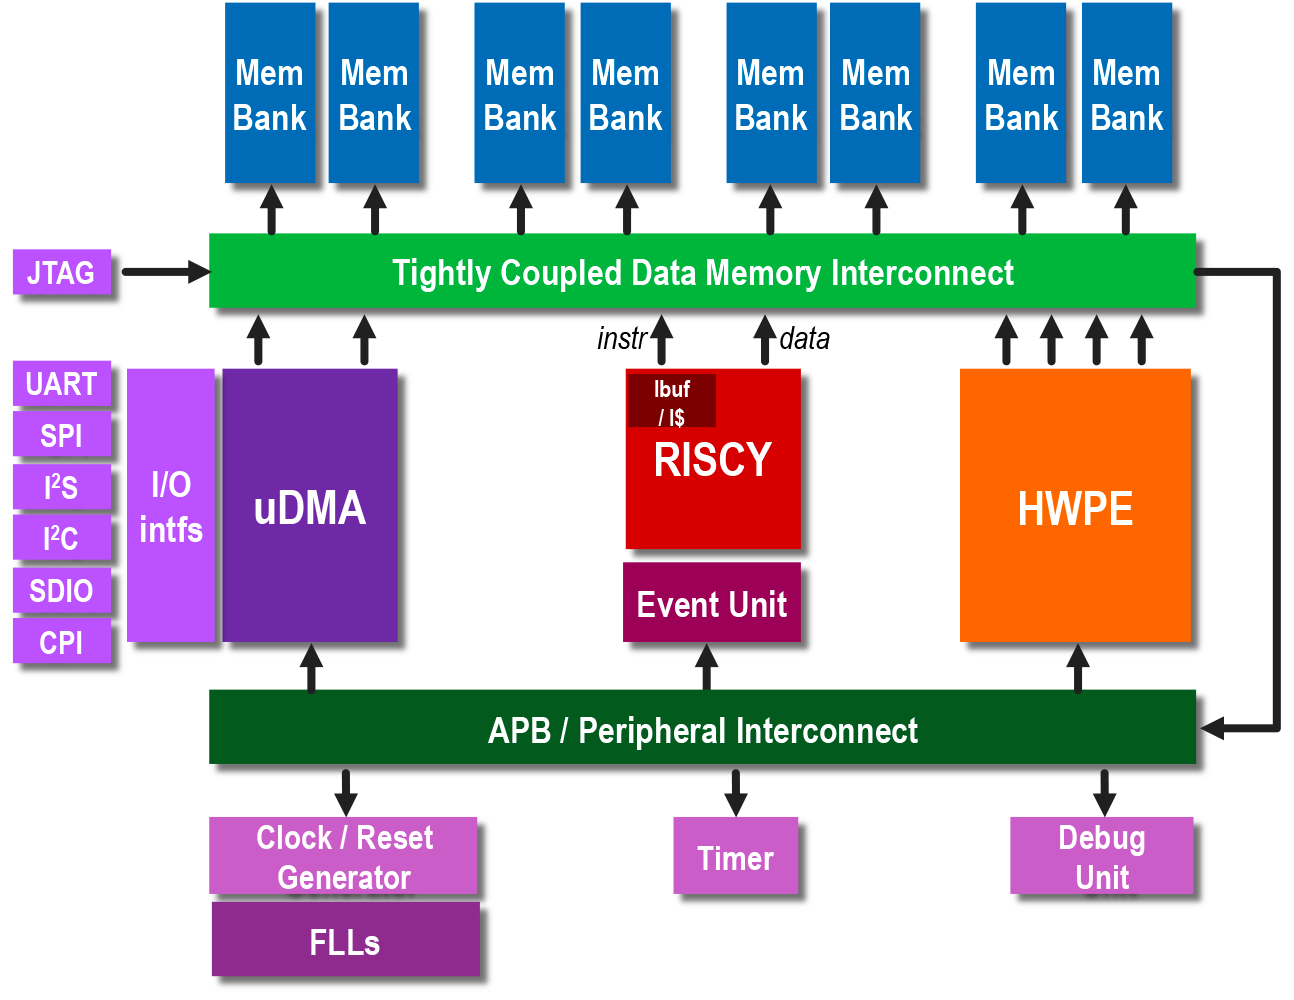
\includegraphics[width=0.6\textwidth]{pulpissimo_arch.png}
	\caption{Architecture of the PULPissimo SoC \cite{pulpissimo}}
	\label{pulpissimo-arch}
\end{figure}

The design is mainly targeting ASIC technology and focussed on maximising energy efficiency. In a \SI{22}{nm} FD-SOI technology, an energy efficiency of \SI{433}{MOPS/mW} has been shown~\cite{Schiavone2018}. The full SystemVerilog RTL code including scripts for simulation and FPGA evaluation is available on GitHub~\cite{pulpissimo}.

\subsubsection*{Hardware Processing Engine (HWPE)}

The PULP hardware processing engine is a quite unique hardware accelerator. As depicted in \Cref{hwpe-arch}, it consists of a data interface, a control interface and the data path. In contrast to most accelerators in literature it neither uses a dedicated accelerator interface in the CPU nor direct memory access (DMA) to get the data to the processing units. Instead, it shares the tightly-coupled data memory with the processor core. The control interface is connected to the peripheral bus and is thus seen as a memory-mapped peripheral by the CPU. It provides configuration registers which can be read and written by the processor.

\begin{figure}
	\centering
	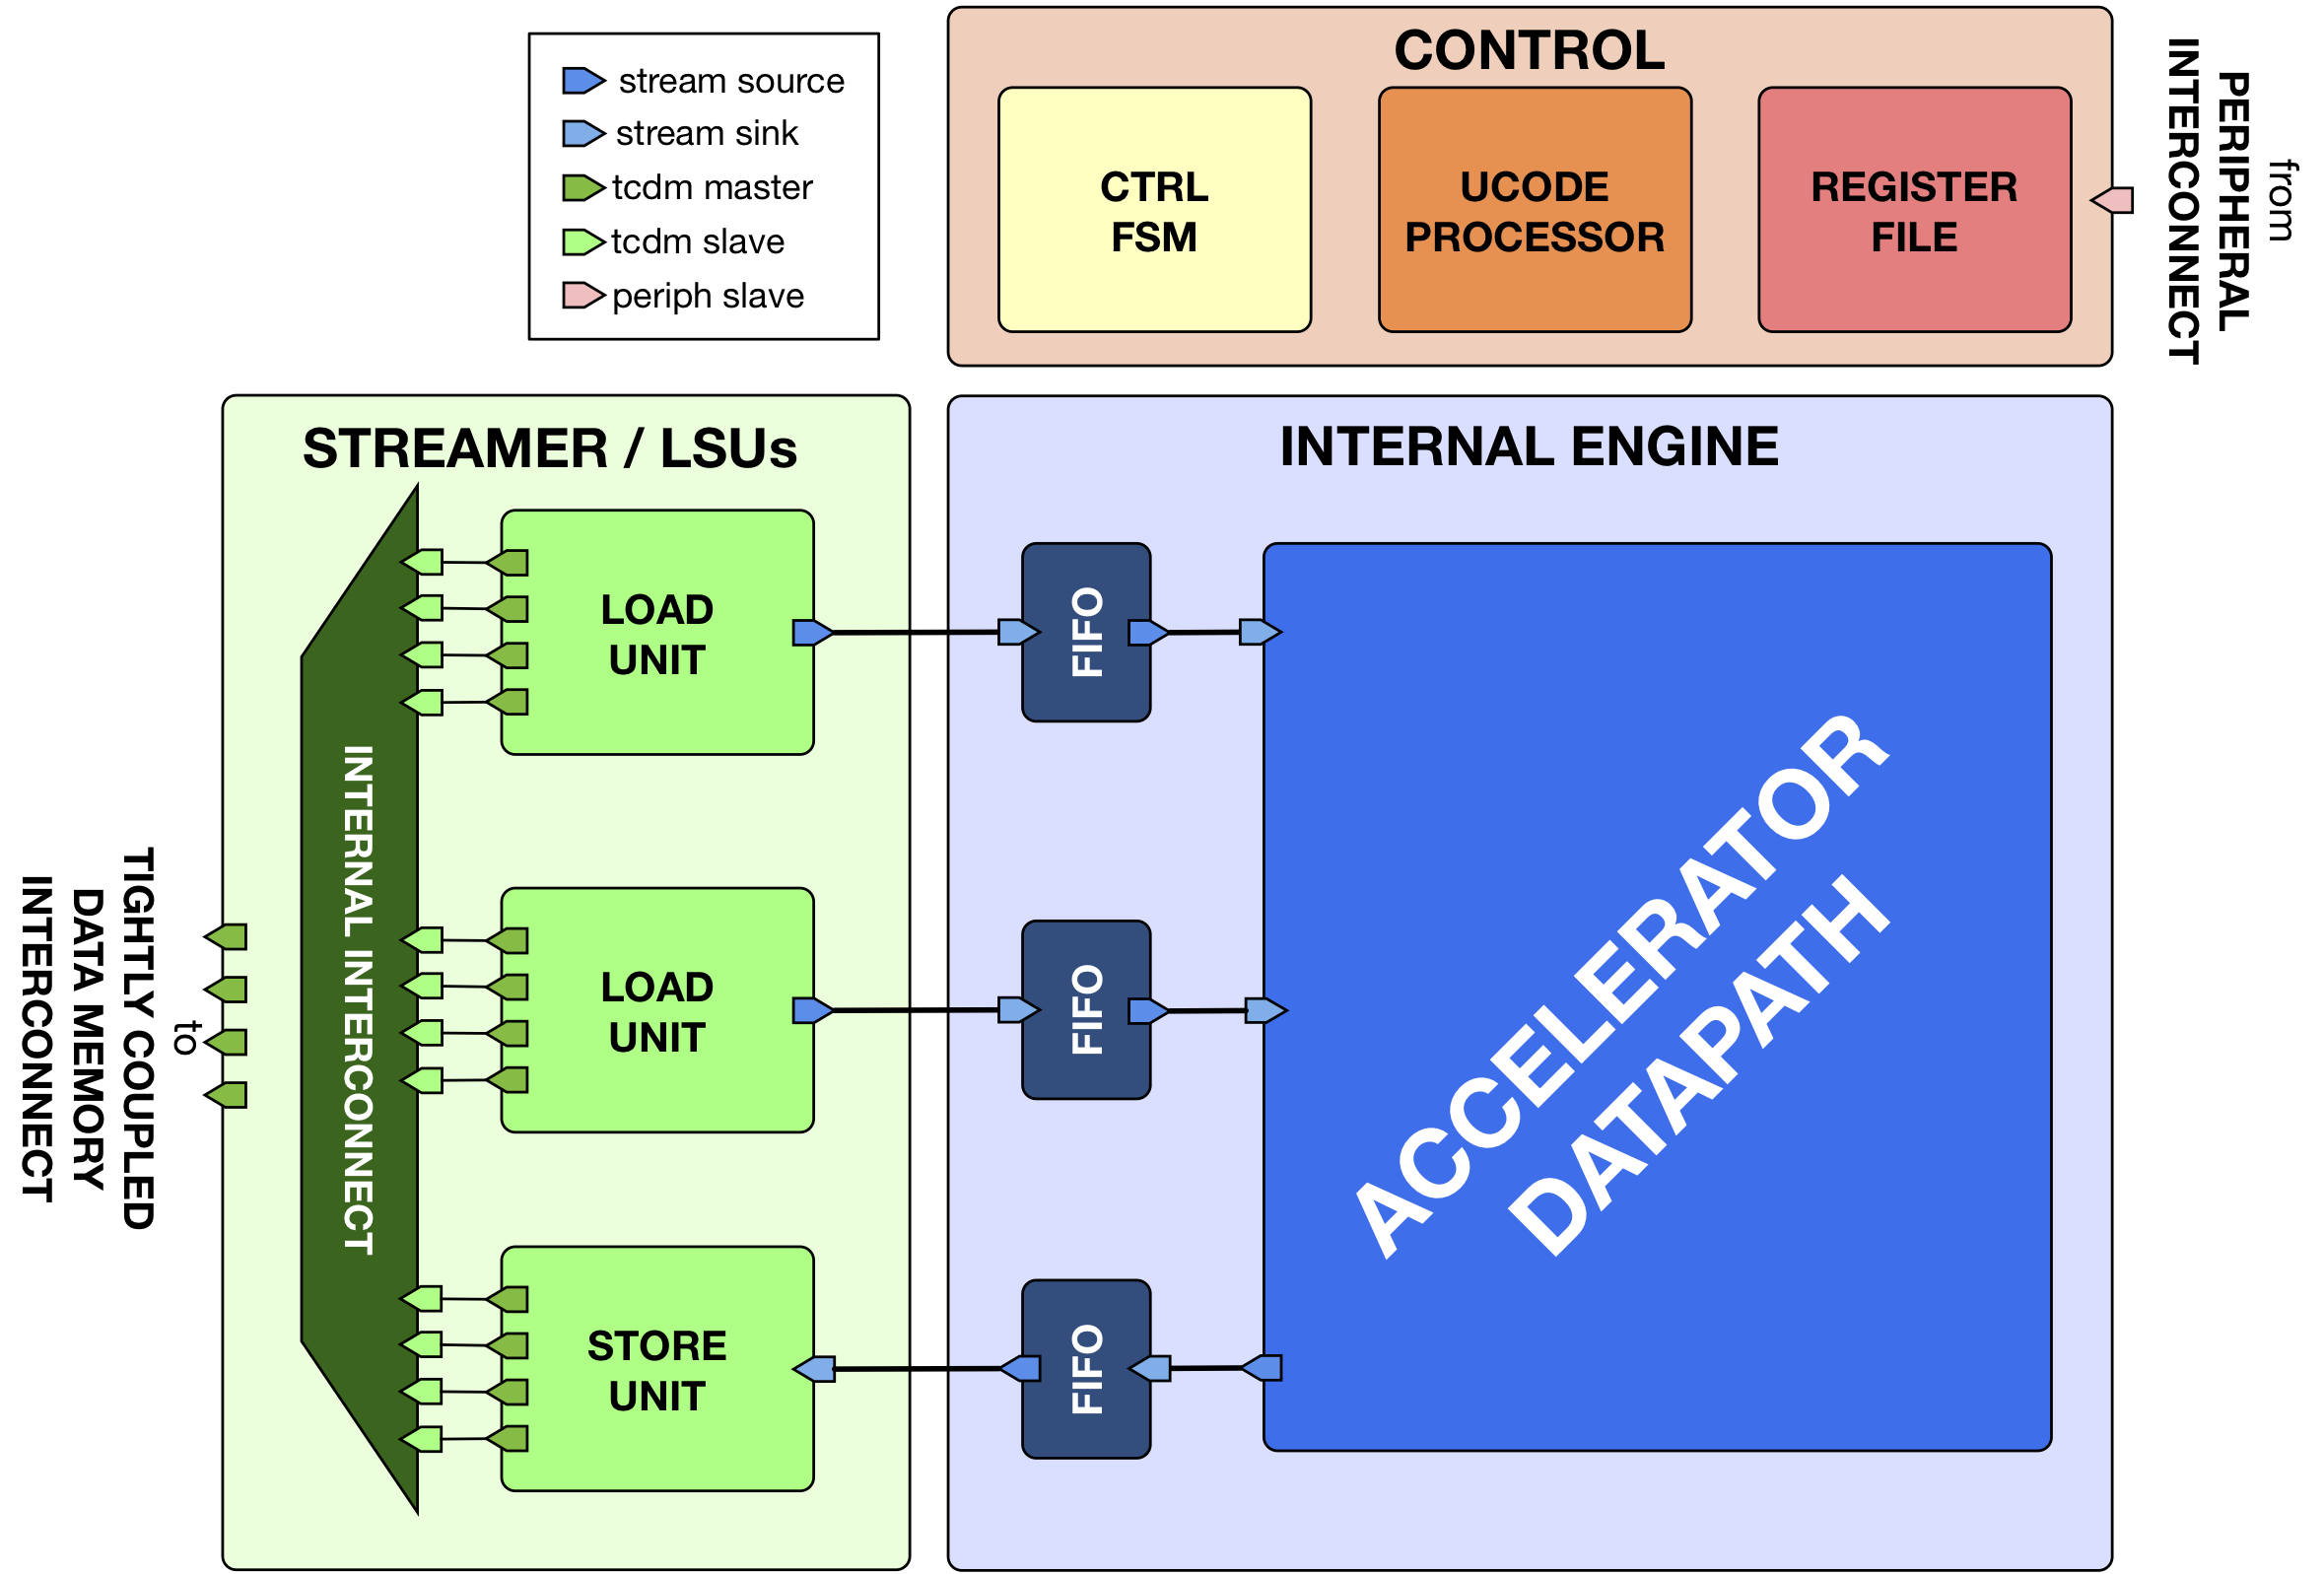
\includegraphics[width=0.65\textwidth]{hwpe.png}
	\caption{Architecture of a PULP Hardware Processing Engine \cite{hwpe}}
	\label{hwpe-arch}
\end{figure}

A typical HWPE operation works as follows. Firstly, the relevant data has to be placed in the shared memory (TCDM). Then, the CPU sets all relevant configuration data (e.g. pointers of source and destination in shared memory, data size, HWPE configuration) via the HWPE´s control interface. Once a HWPE operation is started, it operates fully autonomous and the CPU can perform other computations. After completion, the HWPE triggers an event which can be polled in the CPU or raise an interrupt. The event indicates that the output data is written to the shared memory.

HWPEs are not limited to PULPissimo, but can also be integrated into more powerful SoCs within the PULP project including multicore systems and HPC clusters. Thus, the effort of designing an HWPE can be reused easily. Furthermore, a template HWPE implementing a multiply-accumulate (MAC) engine is available~\cite{hwpe-mac}. This template features a relatively simple data path, but a powerful control interface including a microcode processor and a finite state machine as well as three 32-bit inputs and one 32-bit output. The template is intended as starting point for new HWPEs and alleviates the burden for the developer to implement a device driver and to handle the memory access. The work in this project is based on this template.

\subsection{AES Hardware}

The advanced encryption standard (AES) defines a set of block-cipher algorithms which are also known under their original Dutch name Rijndael. It works on 128-bit data words and uses either 128, 192, or 256-bit keys. The algorithm was designed for straightforward hardware implementation and is one of the most frequently used block ciphers.

In general, AES operates in (mostly) identical rounds (10 for 128-bit keys), each of which consists of different mathematical steps. Hardware designs might implement these operations once and compute the round results sequentially or pipeline them to some extent. Faster implementations consist of several parallel round hardware blocks.

Thus, several hardware implementation of the AES algorithms are available. As this project uses open-source SystemVerilog RTL code, only permissively-licensed open-source (System)Verilog implementations were considered. \Cref{tab:aes_cores} compares the three most relevant IP cores. An edge device requires only encryption capabilities to transfer sensor data in a secure way. Due to size and energy limitations, only AES with 128-bit keys was considered.

\begin{table}[h]
    \centering
    \begin{tabular}{c|c c c}
        \toprule
        IP Core &  \verb|tiny_aes|~\cite{tiny-aes} & \verb|aes_128|~\cite{aes-128} & \verb|secworks_aes|~\cite{secworks-aes}  \\
        \midrule
        Cycles/op &  1 & 12 & 4\\
        Latency (cylces) & 21 & 12 & 14\\
        LUTs & 4588 & 487 & 3327 \\
        Registers & 4474 & 402 & 2990 \\
        BRAM tiles & 68 & 5 & 0 \\
        Max. frequency [MHz] & 375.9 & 180.5 & 124.8 \\
        Decryption & no & yes  & yes \\
        256-bit keys & no & no & yes\\
        \bottomrule
    \end{tabular}
	\caption{Comparison of selected open-source AES IP cores. Resource consumption and clock frequency were obtained with Vivado 2020.2 synthesising for a Nexys~4~DDR evaluation board.}
	\label{tab:aes_cores}
\end{table}

Clearly, the \verb|tiny_aes| core provides the best performance. It is fully pipelined and thus offes the highest throughput and the shortest critical path. In contrast, \verb|aes_128| is a minimalistic implementation that reuses the stages of the AES algorithm to minimise hardware resources. In between, the \verb|secworks_aes| core finds a trade-off and optionally offers features that are not required for this project (decryption and larger keys). Given the energy constraints and the most likely relatively low number of transmissions required, the \verb|aes_128| IP core was selected to be integrated into PULPissimo as HWPE.

\section{Baseline Implementation} \label{sec:implementation}

A first step towards integrating the \verb|aes_128| core into PULPissimo was already taken in a prior course. This report mainly focusses on the new contributions. Still, a wrap-up of the prior work is given in this section for easier understanding.

\subsection{Setup} \label{sec:implementation:setup}

As PULPissimo is written in SystemVerilog and the scripts require either Mentor Questa Sim or Cadence Xcelium, an ICT EDA server was used to run the Mentor toolchain. This required working on the server´s file system and mounting the relevant directories via \texttt{sshfs} on the local machine as all required dependencies for compilation were installed there. As the PULPissimo scripts make use of environment variables frequently, doing so required several scripts enabling a seamless workflow when switching back and forth between the two platforms.

\subsection{Reference Software}

To have a reasonable baseline, a software implementation of the AES algorithm was required. Due to its small code size which perfectly fits microcontroller environments, the Tiny AES in C~\cite{tiny-aes-c} implementation was chosen. It easily compiles for PULPissimo with the PULP SDK and requires only around \SI{2}{kiB} of memory. The software library offers several encryption modes and key sizes. However, for the first version only electronic code book (ECB) encryption capability with 128 bit keys was used. 

\subsection{Hardware Processing Engine}

The design of the AES HWPE supports only 128-bit ECB encryption and is based on the PULP MAC engine template~\cite{hwpe-mac}. It contains the AES IP core as well as units converting the 32-bit memory words to 128-bit AES keys and words (word\_stackers and word\_unstacker). The resulting AES HWPE architecture is depicted in \Cref{hwpe-aes}. The input and output streamers are controlled by the FSM in the control block which uses the registers written by the CPU beforehand. All data path units use a simple ready/valid handshake to allow both forward and backward dependencies, e.g. if the AES unit is busy of no new data is provided by the input streamers yet.

\begin{figure} [h]
	\centering
	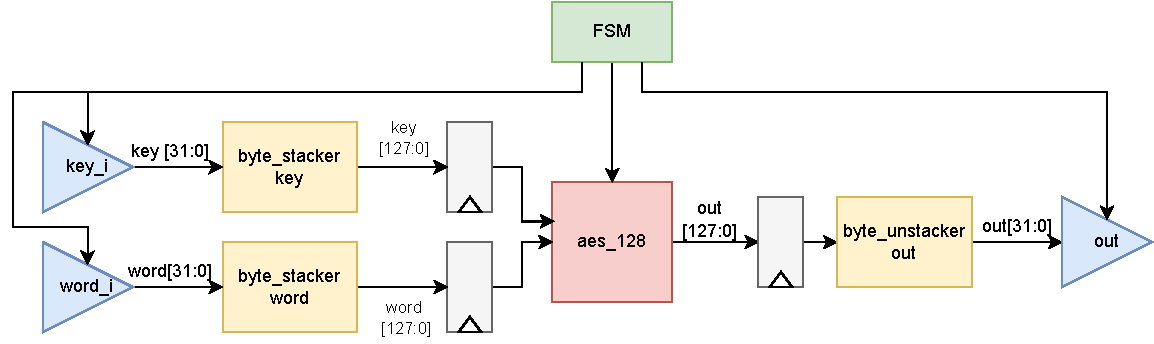
\includegraphics[width=0.95\textwidth]{hwpe_aes.pdf}
	\caption{Block diagram of the implemented AES HWPE}
	\label{hwpe-aes}
\end{figure}

\section{Improved AES Engine} \label{sec:improvements}

The work described from here on was conducted during the SoC Advanced course. Firstly, the AES engine has been improved and demonstrated on an FPGA. Additionally, an ASIC implementation flow was performed. The corresponding results of the latter are described in \Cref{sec:asic}.

\subsection{Register Reduction}

In a first step, the pipelining registers depicted in \Cref{hwpe-aes} were removed. They added area as well as increased the latency without providing any value to the timing behaviour as both the byte\_stacker modules and the AES IP core already provide pipelining registers at their outputs.

\subsection{Cipher Block Chaining}

As the electronic code book encryption mode produces identical output values for identical input blocks, it lacks the so-called diffusion property and is thus not considered safe. Therefore, the AES core was extended to support the cipher block chaining (CBC) mode of operation. Here, the plain text is XOR-connected with the last ciphertext to produce different outputs for identical inputs, s. \Cref{fig:cbc}.

\begin{figure} [h]
	\centering
	
\includegraphics[width=0.65\textwidth]{cbc.png}
	\caption{Cipher block chaining mode of operation \cite{wiki_cbc}}
	\label{fig:cbc}
\end{figure}

Adding CBC support to the AES HWPE requires only small modifications. Firstly, a register storing the last ciphertext is required. Then, a 128-bit XOR block has to be added. The resulting architecture is shown in \Cref{hwpe-aes-update}. As the pipeline features a ready-valid handshake system which is not depicted, some additional handshake signals are required to ensure that each ciphertext is used exactly once. The reset value of the ciphertext register is the initialisation vector (IV), which is hardwired in the current implementation. In principle, it is possible to make the IV configurable via the peripheral bus interface. A further conceivable improvement is a configuration bit that allows switching between ECB and CBC.

\begin{figure} [h]
	\centering
	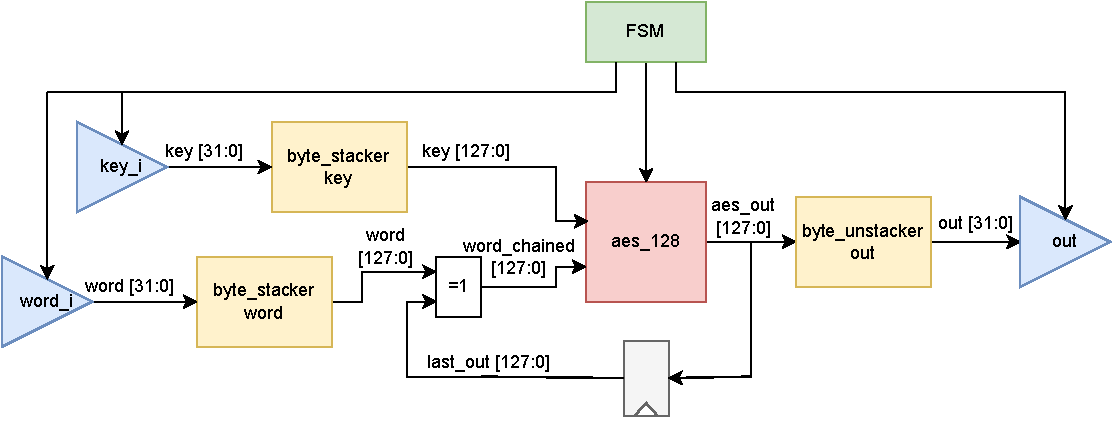
\includegraphics[width=0.95\textwidth]{hwpe_aes_update.pdf}
	\caption{Block diagram of the improved AES HWPE}
	\label{hwpe-aes-update}
\end{figure}

The used reference software implementation \cite{tiny-aes-c} already provides build-in CBC support and thus only a preprocessor flag has to be set. Again, a short self-checking demo application was written both for the PULPissimo CPU using the library and the HWPE. Both use the same set of data from the NIST examples~\cite{NIST}. To make sure the cipher feedback is done correctly, blocks of four encryptions are executed as the output data does not differ between ECB and CBC for a single encryption. In a first step, the HPWE was evaluated in a RTL simulation where both the reference program and the HWPE application yielded the expected results.

\subsection{FPGA Demonstration}

An important part of this project was evaluating the AES HWPE on an FPGA target as FPGA synthesis was not achieved during the prior course. Initially, the selected target was the Digilent Nexys~4~DDR board which is supported by the scripts in the PULPissimo repository. However, the design fills the board almost entirely (s. \Cref{sec:improvements:results}) which makes placement and routing times extremely long. Furthermore, an external JTAG debugger is required to run code on the SoC as the built-in JTAG interface is not supported. Therefore, the Digilent Genesys~2 evaluation board was selected as it features a significantly larger Xilinx FPGA from the same generation and the provided synthesis scripts support its on-board JTAG unit.

As outlined in \Cref{sec:implementation:setup}, a mounted file system was used to work both on the institute's EDA server and a local machine. This however caused problems with Vivado 2020.2 which apparently has issues when running synthesis on mounted files. Thus, a local copy of the files was made to execute FPGA synthesis. Additionally, the FPGA designs use a different top-level file than the simulation model, thus the \verb|ENABLE_HWPE| parameter has to be set again.

Executing an application with PULPissimo on an FPGA requires a debugging session consisting of a debugger (in this case \texttt{gdb}) and an OpenOCD server providing an interface to the on-board JTAG unit. Then, the executable can be flashed onto the FPGA and the output can be observed via UART. Again, the software implementation worked flawlessly. 

\todo{move to other position}However, the issued described in \Cref{sec:asic:verification} were observed on the FPGA demonstrator as well. Thus, the HWPE was only successfully demonstrated after applying the changes required for ASIC synthesis.

\subsection{Results} \label{sec:improvements:results}

\subsubsection{Performance}

Both the reference software implementation and the HPWE program were simulated and the runtimes recorded. All outputs checks passed. As the runtimes for the hardware implementation were hardly measurable from the software, they have been extraced from the waveforms. \Cref{tab:results} compares the software implementation and the HWPE. Clearly, the hardware implementation outperforms the software -- which can not make use of any hardware-accelerated encryption primitives in terms of runtime. The code size decreases for the hardware implementation as the AES functionality (including relatively large look-up tables) is offloaded to hardware. Note that the code size given here is for the full demo program and thus includes not only the AES encryption but also the stimuli and several system routines.

\begin{table}[h]
    \centering
    \begin{tabular}{c|c c}
        \toprule
        & Software & HWPE \\
        \midrule
		Cycles four encryptions & 18300 & 97 \\
		Cycles additional encryption & 4500 & 17 \\
		Relative speed-up & 1  & 264.7 \\
		Code size [bytes] & 10052 & 9096 \\
        \bottomrule
    \end{tabular}
	\caption{RTL Simulation results for different AES CBC implementations.}
	\label{tab:results}
\end{table}

The overhead for the first four encryptions relative to each further (contiguous) operation lies in the control flow. Firstly, a HWPE lock has to be acquired and both the data length and the start bit have to be set (14 cycles). Then, the streamer has to fetch the data from the TCDM (7 cycles). In a next step, the AES engine produces output data and provides them to the streamer (21 cycles). Further data words benefit from pipelining as reading in and writing out can happen simultaneously. Thus, they only take 17 cycles each (if the data is already provided in the TCDM and no memory congestion occurs). Finally, the data is transferred to the memory and the completion event is issued (4 cycles). 

\subsubsection{FPGA Resources}

\Cref{tab:results-genesys} summarises the resource consumption of different entities after synthesis for this target. Clearly, there is still plenty of headroom on the board -- this simplifies placement and routing. The HWPE introduces an overhead of \SI{7.1}{\percent} for LUTs and \SI{7.4}{\percent} for registers respectively. However, the main contributor is not the data path (HWPE engine) but the HWPE streamer which provides the interface to the tighlty-coupled data memory.

\todo{update}
\begin{table}[h]
    \centering
    \begin{tabular}{c|c c c}
        \toprule
        Entity &  Look-up-tables & Registers & BRAM tiles \\
        \midrule
		FPGA &  203800 &  407600 &  445 \\
		PULPissimo & 58656 & 45155 & 144 \\ 
		HWPE Top & 3892 & 3115 & 0 \\ 
		HWPE Ctrl & 172 & 165 & 0 \\ 
		HWPE Streamer & 2151 & 1886 & 0 \\ 
		HWPE Engine & 1569 & 1064 & 0 \\ 
		AES Core & 1247 & 530 & 0 \\ 
		Word Stacker (each) & 26 & 131 & 0 \\ 
		Word Unstacker & 118 & 131 & 0 \\
        \bottomrule
    \end{tabular}
	\caption{Resource consumption of the PULPissimo SoC when synthesised for the Genesys~2 evaluation board.}
	\label{tab:results-genesys}
\end{table}

\pagebreak
\section{ASIC Synthesis} \label{sec:asic}

As the PULP platform is mainly concerned with energy efficiency, the designs are aimed at low-power ASIC technologies (while FPGA is limited to prototyping and demonstration). Therefore, it is interesting to perform ASIC synthesis of the AES engine to obtain comparable area and power figures.

As ASIC implementation is only briefly touched in the TU Wien Embedded Systems curriculum, a major part of the project was getting familiar with the required technologies and tools. Due to their widespread use and availability at the ICT, the Cadence toolchain and the TSMC \SI{65}{nm} technology were used. Further details are discussed in \Cref{sec:asic:tools}.

As the PULPissimo SoC has been taped out several times~\cite{pulp-chips}, the implementation is limited to the AES HWPE. The corresponding flow is outlined in the rest of this section. However, as discussed in \Cref{sec:asic:verification}, the ASIC verification showed some issues in the design which required small design changes which unfortunately limit the design versatility.\todo{reference}

\subsection{Technology and Tooling} \label{sec:asic:tools}

The backend design flow used for this project is based on the Cadence digital implementation toolchain and depicted in \Cref{fig:asic-flow}. Most steps are automated with \texttt{tcl} scripts and \texttt{Makefiles}. After simulation-based RTL verification, the design is synthesised to the technology-specific cells with Genus. The resulting netlist is verified both by simulation and model checking. Then, a layout is generated with Innovus. The final delay-annotated netlist is again verified and can be used for both power estimation with Voltus and static timing analysis (STA) with Tempus.

The design was implemented with TSMC \SI{65}{nm} digital standard cells featuring a cell height of 10 tracks and 6 metallisation layers. To cope with process, voltage, and temperature (PVT) variations, all analyses were conducted for three corners, namely typical (\SI{1.0}{V}, \SI{25}{\degreeCelsius}, normal transistors), best case (\SI{1.1}{V}, \SI{0}{\degreeCelsius}, fast transistors), and worst case (\SI{0.9}{V}, \SI{125}{\degreeCelsius}, slow transistors).

Despite the intention of creating an energy-efficient accelerator, hardly any power management techniques were implemented. Namely, the design neither features clock or power gating nor low-power standard cells. Furthermore, no design-for-test strategies like scan chains were used. This is due to the limited scope of this project. Of course, any silicon implementation of this design should consider making use of those industry-standard techniques.

\begin{figure} [h]
	\centering
	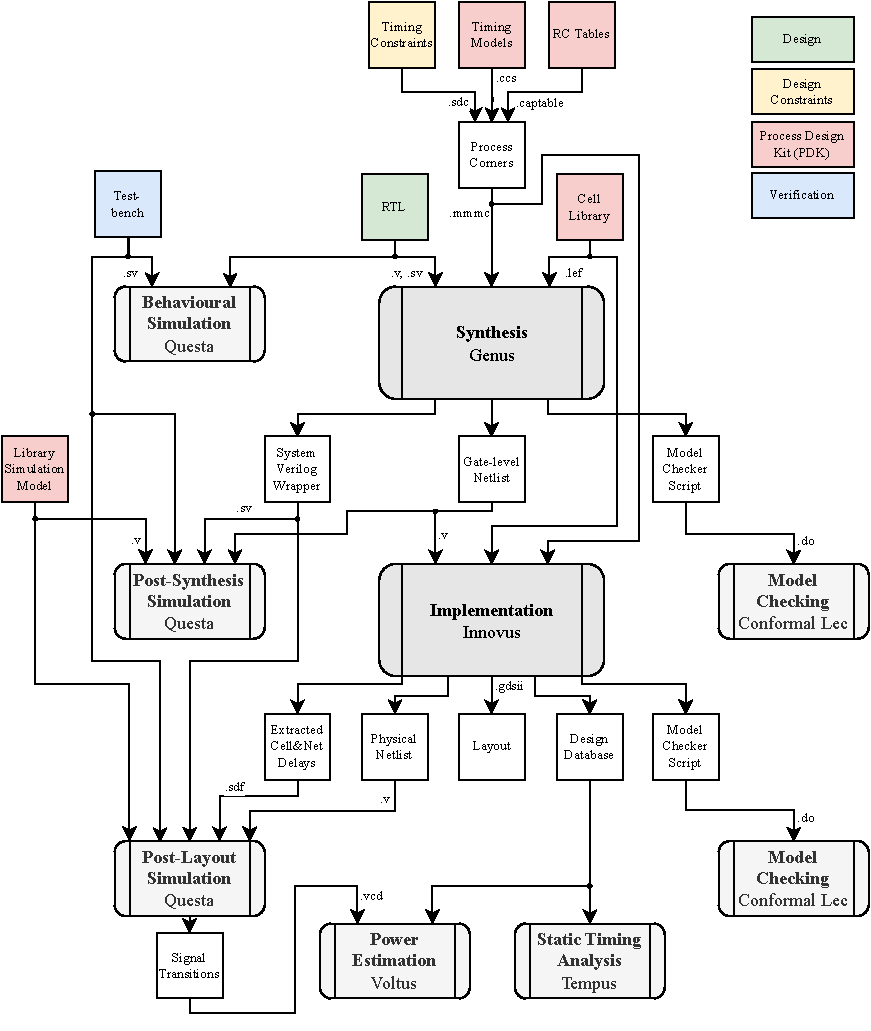
\includegraphics[width=0.86\textwidth]{design-flow.pdf}
	\caption{ASIC design flow used for this project}
	\label{fig:asic-flow}
\end{figure}

\clearpage

\subsection{Synthesis} \label{sec:asic:synthesis}

Before the actual synthesis can take place, the design requires appropriate timing constraints. The clock frequency was iteratively set to \SI{625}{MHz}. Higher frequencies are hardly achievable with the given RTL model. The remaining clock constraints (skew, latency, transition time) were also reduced as far as reasonably feasible. As the reset of the HWPE is asynchronous, all timing arcs starting from this signal are constrained als false paths. Notably the latches in the HWPE control pane do not require false paths as Tempus can calculate timing analyses for latch-based designs.

As the AES HWPE is no self-containing chip but intended to be integrated into a PULPissimo SoC, the input and output pins are assumed to be connected with relatively short connections to other parts of the chip. Therefore, the corresponding delay, driver, and load constraints were inspired by the behaviour of the buffers available in the cell library.

The Genus synthesis flow replaces the RTL model with generic cells, then finds suitable technology-specific cells and finally optimises the resulting netlist for area and timing. As the top-level module is specified in SystemVerilog and netlists are usually defined in Verilog, a SystemVerilog wrapper is required to instantiate the AES HWPE in a verification environment. The module parameters are tied during synthesis, thus the synthesised module has to be instantiated without any parameters.

\subsection{Implementation} \label{sec:asic:impl}

\todo{floorplan}

\todo{placement + power routing}

\todo{CTS}

\todo{routing + optimisation}

\todo{fixing violations}

\todo{filler cells and metal}

\todo{checks}

\todo{output}


\subsection{Verification} \label{sec:asic:verification}

\subsection{Results} \label{sec:asic:results}

\todo{layout image}

\todo{area post synthesis and layout: per entity, physical cells}

\todo{timing incl. critical path, latch issues}

\todo{power consumption: where does the energy go?}

\section{Summary and Outlook} \label{sec:summary}

\clearpage
\sloppy
\printbibliography

\end{document}
